\chapter{Results}

I have tested the two algorithms described in \nameref{chap:design} using the structure given in \nameref{chap:implementation}.\\
There are two major parts which should be analyzed: the correctness of the algorithm and it's running time.

\section{Correctness}

For testing purposes, I have used a database of $500$ images, containing groups of the same image with different watermarks and sizes. I ran the $linear\ algorithm$ in order to form groups of matching images which could be easily checked for similarity. \\

\section{Running time}

To be able to determine the speed of the two presented algorithms I have run them on sets of $5, 10, 20, 50, 200, 350$ and $500$ images. The corresponding running times are shown in Figure~\ref{fig:runtimesBasic}.\\
The red line shows the corresponding running times for the $linear\ algorithm$, while the green one show the times for the $kdtree\ algorithm$. As it can be seen, the $kdtree\ algorithm$ outperformes the linear one, with the same returned image (so it does not give different results). The non-ascending running times of the $kdtree\ algorithm$ can be explained by the fact that the KD-tree data structure is traversed heuristically, so depending on the given input a certain query can execute with varying running times. \\
Of course. the $kdtree\ algorithm$ does require an initialization time, which is the price that has to be paid in order to perform fast queries. Figure~\ref{fig:inittimesBasic} shows the initialization time of an image server which constructs a KD-tree server. As it can be seen, this time grows linearly, but this gets compensated by the small query time. For a $500$-size image set, the initialization of the KD-tree takes $35.476$ seconds, which is less than a query on the same image set using the $linear\ algorithm$, which takes $77.331$ seconds.

\begin{figure}[ht!]
\centering
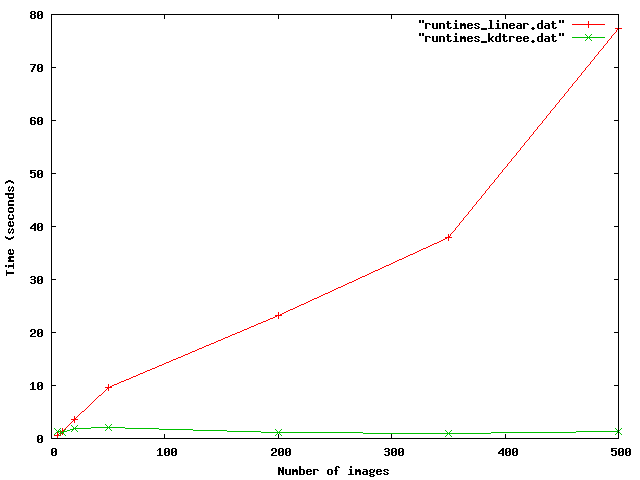
\includegraphics[width=.7\linewidth]{images/runtimesBasic.png}
\caption{Runtime of the two algorithms}
\label{fig:runtimesBasic}
\end{figure}

\begin{figure}[ht!]
\centering
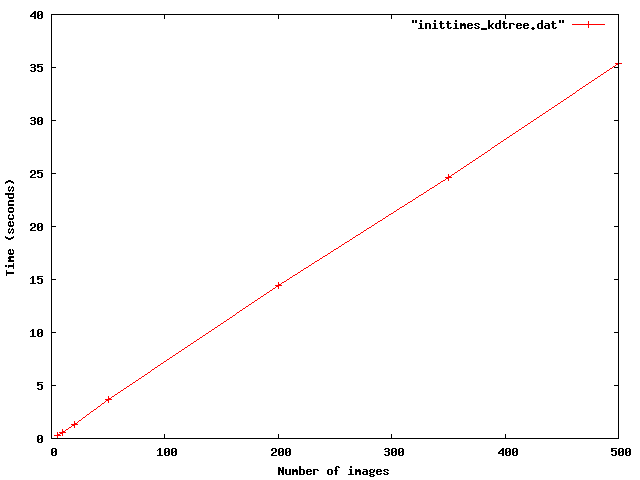
\includegraphics[width=.7\linewidth]{images/inittimesBasic.png}
\caption{Initialization time of a KD-tree server}
\label{fig:inittimesBasic}
\end{figure}